\section{Magnons}

Magnons occur as excitations in spin Hamiltonians describing magnetic systems.

\subsection{The Heisenberg Model}

\begin{figure}[htbp]
    \centering
    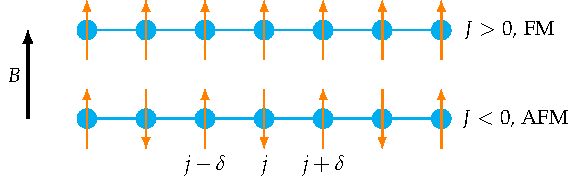
\includegraphics[]{Images/fig-FMAFMHeisenbergchain.pdf}
    \caption{Cartoon depiction of the 1-D Heisenberg chain. For $J > 0$ we have a ferromagnet with aligned spins. For $J < 0$ we have an antiferromagnet with alternating spins. Nearest neighbour spins are coupled, and there is an external magnetic field that affects each spin.}
    \label{fig-FMAFMHeisenbergchain}
\end{figure}

Here, we will discuss the simplest such Hamiltonian describing a magnetic system, the Heisenberg model. It is written as:
\begin{equation}
    H = -J\sum_{j, \delta}\v{S}_j \cdot \v{S}_{j+\delta} - 2B\sum_j S_j^z
\end{equation}
Where the first term represents the coupling between spins, parameterized by a coupling constant $J$ (where $J > 0$ gives rise to a ferromagnet and $J < 0$ to an antiferromagnet), and the second term represents the contribution from an external magnetic field with strength $B$. Note that this Hamiltonian is completely invariant under the choice of $z$-axis; more formally, it is invariant under $SU(2)$ rotations.

Note that $\v{S}_j = (S_j^x, S_j^y, S_j^z)$ is a spin operator at site $j$ that obeys:
\begin{equation}\label{eq-spinalgebra}
    [S^\alpha_i, S^\beta_j] = i\delta_{ij}\e^{\alpha\beta\lambda}S^\lambda_j
\end{equation}
The second property is that $\v{S}_j \cdot \v{S}_j$ has eigenvalues $s(s+1)$ where $s = \frac{1}{2},1,\frac{3}{2},\ldots$. Note that despite its simple form, the Heisenberg Hamiltonian is generally not solvable; it is only analytically solvable (in a difficult method; Bethe ansatz) in 1D and treatable via approximate methods in higher dimensions. In our class, we will solve the 1D chain approximately

\subsection{Magnon Variables}
We will proceed with the approximate solve by transforming into ``magnon variables'' using the Holstein-Primakoff transformation. Recall the raising/lowering operators:
\begin{align*}
    S_i^\pm = S_i^x \pm i S_j^y
\end{align*}
In Holstein-Primakoff, these operators are expressed using bosonic operators:
\begin{equation}\label{eq-HPtransSplusminus}
    \begin{split}
        S_j^+ &= \sqrt{2S}(1 - n_j/2s)^{1/2}a_j
        \\ S_j^- &= \sqrt{2S}a_j^\dag(1-n_j/2s)^{1/2}
    \end{split}
\end{equation} 
with $[a_j, a_k^\dag] = \delta_{jk}$ and $n_j = a^\dag_j a_j$ the number operator. This seems like a strange, nonlinear transformation, but in fact is necessary to satisfy the SU(2) algebra. Raising/lowering operators allow for raising/lowering the states to infinity, but spins have a finite number of states. For certain eigenvalues, $n_j = 2s$ and so we get zero, i.e. we cannot raise the spin state beyond its maximal value. We have $S^+, S^-$, and to finish the set we have:
\begin{equation}\label{eq-HPtransSz}
    S_z = s(s-1) - (S^x)^2 - (S^y)^2 = s(s-1) - \frac{1}{2}(S^+S^- + S^-S^+) = S - a_j^\dag a_j
\end{equation}

Note that the transformations Eqs. \eqref{eq-HPtransSplusminus}, \eqref{eq-HPtransSz} is \emph{exact} in that it satisfies the original spin algebra\footnote{``It is a bitch to work out.'' - Marcel Franz 2022} Eq. \eqref{eq-spinalgebra}. However, it is not very useful as written due to the $\sqrt{}$ in \eqref{eq-HPtransSplusminus}. However, it is useful when we study excited states close to the ordered ground state of $H$, where the spins are completely saturated. In this limit, we assume that only a small number of spins deviate from their perfect arrangement, that is:
\begin{equation}
    s - \avg{S_j^z} = \avg{a_j^\dag a_j}
\end{equation}
is small, and so:
\begin{equation}
    \frac{\avg{n_j}}{s} \ll 1.
\end{equation}
We can therefore expand the square roots in Eq. \eqref{eq-HPtransSplusminus}:
\begin{equation}
    \begin{split}
        S^+ &= \sqrt{2S}\left[a_j - \frac{n_j}{4s} + \ldots \right]
        \\ S^- &= \sqrt{2S}\left[a_j^\dag - a_j^\dag \frac{n_j}{4s} + \ldots \right]
    \end{split}
\end{equation}
and retain only the leading term in this expansion, and write:
\begin{equation}
    \v{S}_i\v{S_j} = \frac{1}{2}(S_i^+ S_j^- + S_i^-S_j^+) + S_i^z S_j^z \approx s(a_i^\dag a_j + a_i a_j^\dag + s - n_i - n_j)
\end{equation}
from here, the ferromagnetic and anti-ferromagnetic lines diverge, so let's analyze the two cases separately.

\subsection{Ferromagnetic Case}
Here we have $J > 0$, and we write the Hamiltonian as:
\begin{equation}
    H = -JS\sum_{\avg{i, j}}\left(a_i^\dag a_j + a_i a_j^\dag + s - n_i - n_j\right) - 2V\sum_j (s - n_j)
\end{equation}
where $\avg{i, j}$ means that $i, j$ are nearest neighbour sites. We can solve this by Fourier transforming:
\begin{equation}
    \begin{split}
        b_k &= \frac{1}{\sqrt{N}}\sum_j e^{i\v{k}\cdot \v{r}_j}a_j
        \\ b_k^\dag &= \frac{1}{\sqrt{N}}\sum_j e^{-i\v{k}\cdot \v{r}_j}a_j^\dag
    \end{split}
\end{equation}
The momentum-space $H$ assumes the form:
\begin{equation}
    H = -JNzs^2 - 2BNs + \mathcal{H}_0 + \mathcal{H}_1
\end{equation}
where $z$ denotes the coordination number (the number of nearest neighbours) and:
\begin{equation}
    \mathcal{H}_0 = \sum_k \left(2Jzs(1 - \gamma_k) + 2B\right)b_k^\dag b_k
\end{equation}
with $\gamma_k = \frac{1}{z}\sum_{\gv{\delta}}e^{i\v{k}\cdot\gv{\delta}}$. If we had a two-dimensional square lattice, then the $\gv{\delta}$ vectors would be as follows:

\begin{figure}[htbp]
    \centering
    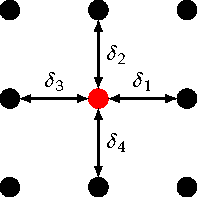
\includegraphics[]{Images/fig-2dsquarelatticedeltas.pdf}
   
    \caption{The four $\gv{\delta}$ vectors for the 2D square lattice. Each atom has neighbours at $\delta = \pm \xhat$, $\delta = \pm \yhat$.}
    \label{fig-2dsquarelatticedeltas}
\end{figure}

Note that this form of $\mathcal{H}_0$ is valid for lattices with an inversion center which implies $\gamma_\v{k} = \gamma_{-\v{k}}$. Without this condition the form of $\mathcal{H}_0$ would be more complicated. One way to think about this is a lattice has an inversion center if for every lattice site, there is both a $\gv{\delta}$ and $-\gv{\delta}$ nearest neighbour. This would not be the case (e.g.) for a honeycomb lattice.

$\mathcal{H}_1$ contains higher order terms in $b_k, b_k^\dag$ and represents magnon interactions.

The situation is analogous to phonons; we made a harmonic approximation, which gave us a nice quadratic Hamiltonian. The higher order terms represented interactions of the phonons. The mechanics is different here but the idea is the same; we have a ``nice'' quadratic Hamiltonian $\mathcal{H}_0$ and then the higher order terms in $\mathcal{H}_1$ representing magnon interactions. Similar to phonons where the harmonic approx was sufficient to describe lattice vibrations but not expansions, we will find that thermodynamics is described well by the lower-order expansion, but (e.g.) thermal conduction will require the higher order terms to analyze.

We write things suggestively as:
\begin{equation}
    \begin{split}
        \mathcal{H}_0 &= \sum_k \omega_k n_k
        \\ \omega_k &= 2Jsz(1 - \gamma_k) + 2B
    \end{split}
\end{equation}
where $\omega_k$ is the magnon spectrum. This tells us about the low energy excitations. 

\subsection{An Example: Cubic Lattice in 3D}
In this example, we have:
\begin{equation}
    \gv{\delta} = \pm a\xhat, \pm a\yhat, \pm a\zhat.
\end{equation}
So then:
\begin{align*}
    z(1-\gamma_\v{k}) = 6 - \sum_{\gv{\delta}}e^{i\v{k} \cdot \gv{\delta}} = 2(3 - \cos(ak_x) - \cos(ak_y) - \cos(ak_z))
\end{align*}
We are interested in the low-temperature/energy and hence long wavelength excitations, so $ka \ll 1$ and so we can expand $\cos(k_ia) \approx 1- \frac{1}{2}k_i^2 a^2$. We then find:
\begin{equation}
    \omega_k \approx 2B + 2Js(ka)^2
\end{equation}
note that the same result holds for FCC and BCC lattices. At zero magnetic field, the magnons exhibit particle like spectra:
\begin{equation}
    \omega_k = \frac{k^2}{2m^*}, \quad m^* = \frac{1}{4Jsa}
\end{equation}
for conventional ferromagnets, it is found that $m^* \approx 10m_e$.

To find the magnon heat capacity, we take $\omega_k = Dk^2$ with $D = 2sJa^2$ and calculate the internal energy $U(T)$:
\begin{equation}
    \begin{split}
        U(T) = \sum_\v{k}\omega_\v{k}\avg{n_\v{k}}_T &= \sum_\v{k}\frac{\omega_\v{k}}{e^{\beta\omega_\v{k}} - 1}
        \\ &= \frac{1}{(2\pi)^3}\int_{\abs{\v{k}} < k_{max}} d^3k \frac{Dk^2}{e^{\beta Dk^2} - 1}
        \\ &= \frac{(k_B T)^{5/2}}{4\pi^2 D^{3/2}}\int_0^{x_m}dx \frac{x^{3/2}}{e^x - 1} \quad x = \beta Dk^2, x_m = D\beta k^2_{max}
        \\ &= \frac{0.45}{\pi^2}\frac{(k_B T)^{5/2}}{D^{3/2}}
    \end{split}
\end{equation}
The integral is dimensionless, so the temperature dependence is entirely in the prefactor. In the last line we have taken the $x_m \to \infty$ to carry out the integral, an approximation that is valid at low temperatures. From this we easily obtain the heat capacity:
\begin{equation}
    C_V = \dod{U}{T} = 0.113k_B(k_B T/D)^{3/2}
\end{equation}
we have another different temperature dependence of the heat capacity! For electrons, $C_V \sim T$, for phonons, $C_V \sim T^3$, and for magnonons, we have $C_V \sim T^{3/2}$. This suggests that if we have an insulating (i.e. no electronic contribution) antiferromagnet, to observe $C_V$ we include a phonon contribution $\sim bT^3$ which means that:
\begin{equation}
    C_V^{tot} = cT^{3/2} + bT^3
\end{equation}
we can then plot $C_V^{tot}/T^{3/2}$ vs. $T^{3/2}$, which gives us a straight line with intercept $c$ as:
\begin{align*}
    \frac{C_V^{tot}}{T^{3/2}} = c + bT^{3/2}.
\end{align*}

One last comment: The midterm will cover what was covered today, the last bit covered next day, and a reading assignment on antiferromagnetic magnons which is on pages 58-62 on the handout.
